\documentclass[letterpaper,10pt,titlepage,journal,compsoc,draftclsnofoot,onecolumn]{IEEEtran}
\linespread{1}
\newcommand\tab[1][1cm]{\hspace*{#1}}
\usepackage{graphicx}                   
\graphicspath{{images/}}                     
\usepackage{amssymb}                                         
\usepackage{amsmath}                                         
\usepackage{amsthm}                                          

\usepackage{alltt}                                           
\usepackage{float}
\usepackage{wrapfig}
\usepackage{color}
\usepackage{url}
\usepackage{listings}

\usepackage{balance}
\usepackage[TABBOTCAP, tight]{subfigure}
\usepackage{enumitem}
\usepackage{pstricks, pst-node}

\usepackage{geometry}
\usepackage{titling}
\geometry{textheight=8.5in, textwidth=6in}



\newcommand{\cblue}[1]{{\color{blue}#1}}

\usepackage{hyperref}
\usepackage{geometry}

\def\name{Tyler Jones}


%% The following metadata will show up in the PDF properties
\hypersetup{
  urlcolor = black,
  pdfauthor = {\name},
  pdfkeywords = {cs462 ''Senior Capstone''},
  pdftitle = {CS 462 Senior Capstone: Progress Report},
  pdfsubject = {CS462 Senior Capstone},
  pdfpagemode = UseNone
}

\title{Investment Performance Mobile App: Spring Term Progress Report}
\author{Tyler Jones, Aviral Sinha, Sam Cooney}

\begin{document}
\begin{titlingpage}
    \maketitle
	\centering{}
    \begin{abstract}
        
     The purpose of the following document is to review and discuss the current state of our investment performance mobile application as of week 6 of Spring Term. Our group will break down the struggles that we faced with the project as individuals, as well as struggles with the project overall.
        
    \end{abstract}
\end{titlingpage}

\newpage

\tableofcontents{}

\newpage

\section{Introduction to Project}

\tab Our project is an investment performance mobile application. Our main goal with this application is to provide users with a way to enter and track the progress of their investments, so they can gain unique financial insight about the quality of said investments. Typically, through a brokerage, for example, users may only see what investments they have, and they are not always given a composite performance, as is the goal with our project. We aim to give the user a metric for both their entire investment portfolio, as well as the ability to drill down into individual investments for a more localized look. At the beginning of development, we sat down as a group and went over the pieces of the project and what would be a good way to breakdown the work. Essentially, we decided that the project could be divided into 3 major components, being the API, the development of the UI, and the backend/database/console application. As will be discussed in this progress report, Avi has taken the lead on the API, Sam on UI development, and Tyler on the backend/database/console application.

\section{Sam Cooney - User Facing Logic and Interface}

For this project, I focused on the development of the mobile application's front end and the logic to support it. Writing in C\# using Xamarin.Forms libraries to support the applications abilities
was completely new to me, but it turned out very exciting. Creating all the different pages and UI elements that lived on them was a difficult but interesting task, that streched my engineering knowledge to try and solves issues and limitations that were brought up by Xamarin.Forms. Overall, the UI turned out very clean and simplistice for the application. There were issues that had to deal with the differences that Xamarin.Forms creates between the iOS and Android versions but we decided that having a single code base was more important than making one platform match the other. If we matched the UI's it would require having two separate codebases, which having a single codebase was one of the key inspirations and requirements for the project.

Currently the front end is completely implemented and works very well on the Android device. There are some issues but these arrise from things like errors in API limits from AlphaVantage, and inconsistency in data provided by Last10k. However, these issues are with the tools we chose to use in the beginning of the project, and if we knew now what we knew then, we would have chosen different tools for those parts of the project as the impact on the application is large.

\begin{figure}[h]
   \caption{Portfolio View Example}
   \centering
   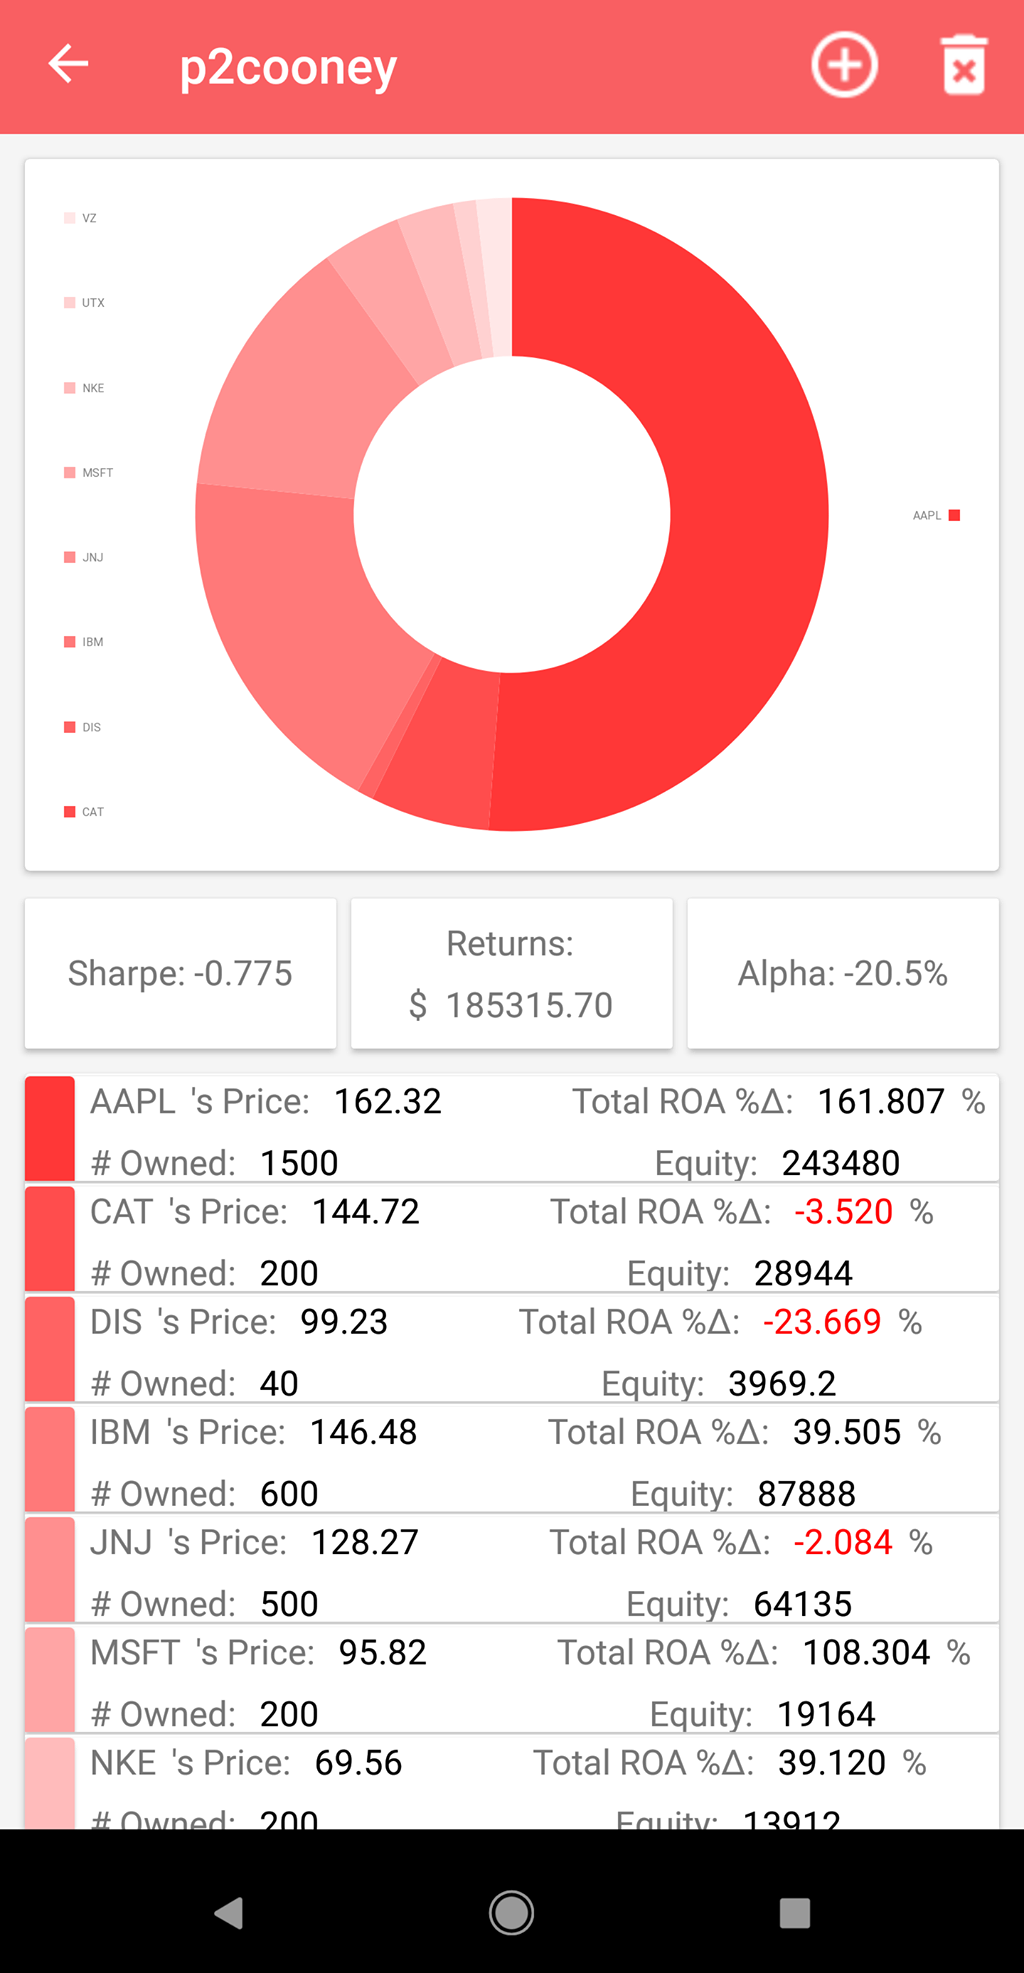
\includegraphics[scale=.15]{spring_portfolio_screenshot}
\end{figure}

Figure 1 is an example of the Portfolio view of the application, where a user can view their created portfolios, review provided analytical data, add new assets, or delete the portfolio. This is where we pictured the user to spend most of the time, so a lot of my focus was on trying to make the elements simplistic, yet still retaining enough information regarding the portfolio and the assets inside it. We ended up using micro charts to create the donut graph pictured above, which is the portfolio split into segments based on the equity of each asset. We decided to go with a red to white fade of color for the graph, as our client requested us to use their company colors "Red, Black, White" at the time, which is a theme I stuck with when designing the UI.

\begin{figure}[h]
   \caption{Asset View Overview}
   \centering
   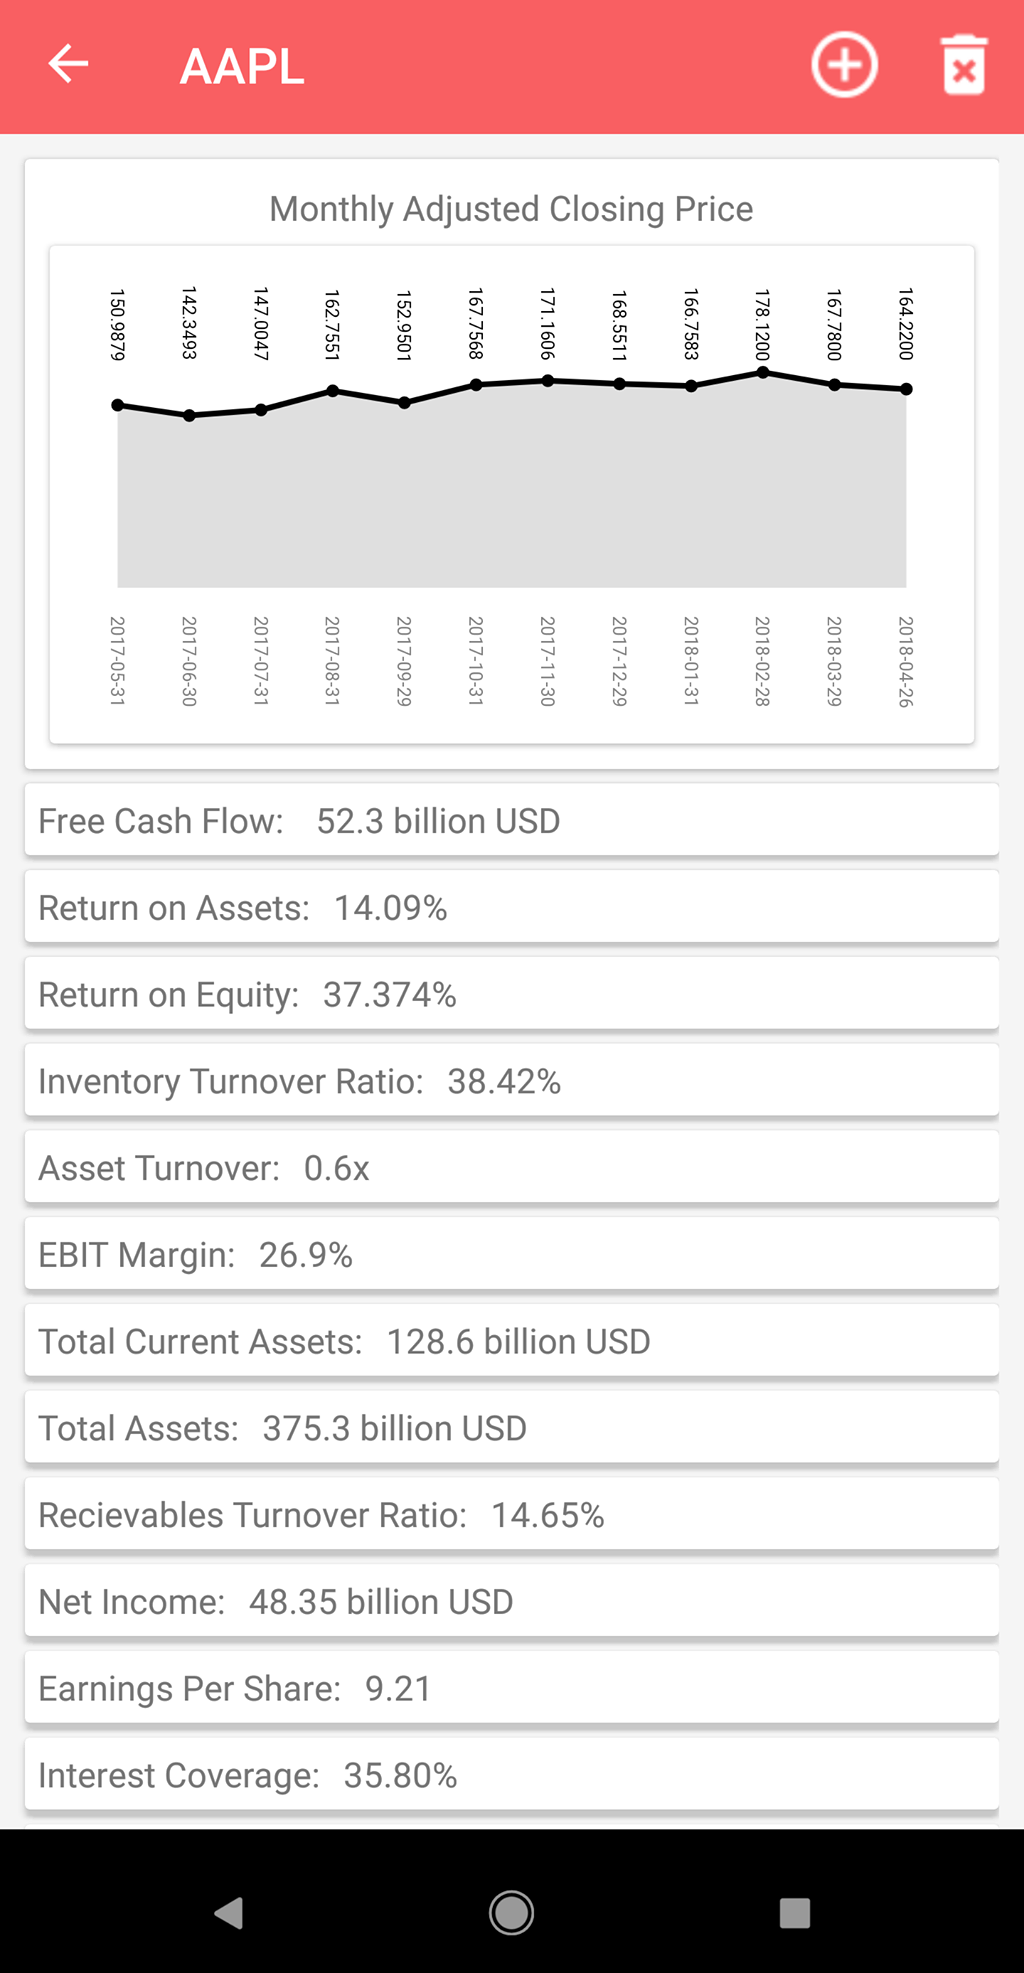
\includegraphics[scale=.15]{spring_asset_screenshot}
\end{figure}

The asset view is where we assume the users will spend the second most time, and as such, the goals for the portfolio view and this view, were the same. I created the cells for the data so the user could quickly index each piece of information quickly and always know where each ratio would be when they opened the page. The bar graph displays the monthly closing price of the stock for the last 12 months, and sticking with the red, black, and white theme, we chose black for this graph to help differentiate it even more from the previous page. Users can also add more of this exact type of stock here as well as delete this individual asset.

\subsection{What's left to do}

The remaining work for my portions are all strech goals and bug fixing. Trying to allievate some of the issues brought on by the UI's, assisting with removing hardcoded parts of the business logic, adding in dynamic drop down boxes for tickers, and dynamic updating for deleting of objects.

\subsection{Problems impeding progress}

Xamarin.Forms does not have the full functionality that each individual native UI provides which proved to be a larger issue than we anticipated. It prevented me from meeting a few strech goals this term so far as the elements did not have the support from Xamarin.Forms to behave in the way that I was requiring.

\section{Avi Sinha - APIs and Business Logic}

\subsection{Description of Current Status}

The project is currently right at release in terms of all the work we set out to complete when beginning development in January. The UI has been fully developed to what is comparable to other brokerage applications currently on the market like Robinhood or Merrill Edge. Like described in the last progress report mid development we made the switch from Quandl to Alpha Vantage and Last10k for our financial data. Alpha Vantage would output the specific stock prices and time series data which was used by Tyler do Portfolio level calculations like the sharpe ratio, overall returns, and then the Alpha of the portfolio. Last10k was used for more asset specific details that we need to show for each company. Currently we have our application displaying the monthly adjusted closing price in a graph provided from the AlphaVantage data and then we have 13 financial ratios showing the viability of owning that security. Last10k provided an intuitive API that allowed me to get all the necessary calculations and ratios needed to show the user an in depth look at the stock. The ratios that are sourced from Last10k are as follows: Free Cash Flow, Return on Assets, Return on Equity, Inventory Turnover, Asset Turnover, EBITDA Margin, Total Current Assets, Receivables Turnover, Net Income, Earnings Per Share, Interest Coverage, Tax Rate, and the Revenue. These values are then taken to the database server and from there the mobile application will pull everything to display on the asset details page for each stock. With the completion of all these parts of the project we have effectively finished all the main requirements that are needed to our end product successful. 

 
\subsection{What's left to do}

For what we have to do there is still some work that needs to be done with UI on the iOS side. We have made the Android version our priority the version we show at expo because of the issues we have faced with xamarin where the shared codebase is making the iOS version look a bit clunky. Once that is completed we will refine any other parts of the application where problems arise. Most of is basically complete now but if any problems arise we have between now and expo to fix them and get it ready for presentation. 
 
\subsection{Problems impeding progress/Solutions}

Our biggest problem that has come up between now and the last progress report is that our client has departed from the project. Being the second time this has happened we weren’t too surprised as from what we have gotten from this is that HedgeServ is going through a lot of restructuring. While we had gotten a new client from the company last time this happened. This time around our previous client let us know that they won’t be a replacement as the project is nearing an end. Luckily our project is essentially dictated by how well we meet our requirements the loss of the client this time around didn’t hurt development too much other than the loss of someone who could give proper financial advice on some of the business logic. We resolved this by getting advice from Kirsten who assured us that everything is fine and happens regularly. We were able to get regular advice from her regarding some parts of the project that would normally be topics of discussion with our client. Other problems included just some issues we had with the integrating everything together from the console application to the UI to the APIs that were used with everything. 

\subsection{Other relevant/interesting information about project}
Below are some relevant pieces of code from the development of the Last10k API data retrieval and how it goes from the database to the actual mobile application. 

The following code sample is from the console application where the data is pulled from Last10k's specific API call for ratios. There I parse the relevant ratios I need as out of the 30 they offer I only need around 13 of them. From here I then have it stored onto the OSU database. 

       \begin{lstlisting} 
       static async void MakeRequest()
        {
            var client = new System.Net.Http.HttpClient();
            var queryString = System.Web.HttpUtility.ParseQueryString(string.Empty);
            client.DefaultRequestHeaders.Add("Ocp-Apim-Subscription-Key",
            "ced63a48eaa34a288772c71c62da184a");

            var uri = "https://services.last10k.com/v1/company/ratios?";

            var response = await client.GetAsync(uri);
        }
    }
       
       \end{lstlisting} 
       
      This establishes the connection with the API where we specifically call the ratios that are stored in their database. Next the data is parsed in pretty straightforward way where I call each of the ratio names as such and then return their outputs. 
      
      \begin{lstlisting}
      internal class Ratios
    {
        public string Ticker { get; set; }
        public string InventoryTurnover { get; set; } 
        public string ReturnOnAssets { get; set; }
        public string ReturnOnEquity { get; set; }
        public string EBTMargin { get; set; }
        public string AssetTurnover { get; set; }
        public string TotalAssets { get; set; }
        public string ReceivablesTurnover { get; set; }
        public string NetIncome { get; set; }
        public string EarningsPerShare { get; set; }
        public string InterestCoverage { get; set; }
        public string TotalCurrentAssets { get; set; }
        public string TaxRate { get; set; }
        public string FreeCashFlow { get; set; }
        public string Revenue { get; set; }


        public override string ToString()
        {
            return $"{Ticker,20}
                     {InventoryTurnover} 
                     {ReturnOnAssets} 
                     {ReturnOnEquity} 
                     {EBTMargin} 
                     {AssetTurnover} 
                     {TotalAssets} {
                     ReceivablesTurnover} 
                     {NetIncome} 
                     {EarningsPerShare} 
                     {InterestCoverage} 
                     {TotalCurrentAssets} 
                     {TaxRate} 
                     {FreeCashFlow} 
                     {Revenue}  "; 
            }
    }
    
      \end{lstlisting} 
      
After this is all done in the console application I then take the data from the API which has been stored on our ENGR database use that to display it on our mobile application.

     \begin{lstlisting} 
      string Url = "http://web.engr.oregonstate.edu/~jonesty/api.php/Investments";

            string content = await client.GetStringAsync(Url);
            JArray investments = JArray.Parse(content);

            if (investments.Count == 0)
            {
                return null;
            }
            else
            {
                for (var i = 0; i < investments.Count; i++)
                {
                    CompanyInfo info = new CompanyInfo();
                    //tempPortfolio.Owners.Add((string)data[i]["username"]);
                    info.tickersymbol = ((string)investments[i]["tickersymbol"]);
                    info.currentprice = (double)investments[i]["currentprice"];
                    info.ReturnOnAssets = (double)investments[i]["ReturnOnAssets"];
                    info.ReturnOnEquity = (double)investments[i]["ReturnOnEquity"];
                    info.EBTMargin = (double)investments[i]["EBTMargin"];
                    info.AssetTurnover = (double)investments[i]["AssetTurnover"];
                    info.ReceivablesTurnover = (double)investments[i]["ReceivablesTurnover"];
                    info.NetIncome = (double)investments[i]["NetIncome"];
                    info.EarningsPerShare = (double)investments[i]["EarningsPerShare"];
                    info.InterestCoverage = (double)investments[i]["InterestCoverage"];
                    info.TotalCurrentAssets = (double)investments[i]["TotalCurrentAssets"];
                    info.InventoryTurnover = (double)investments[i]["InventoryTurnover"];
                    info.TaxRate = (double)investments[i]["TaxRate"];
                    info.FreeCashFlow = (double)investments[i]["FreeCashFlow"];
                    info.Revenue = (double)investments[i]["Revenue"];

                    infoList.Add(info);
     
     \end{lstlisting} 
     
     After calling the information from our database it would then be displayed using both a xaml file and xaml.cs file which contains most of the work required for both portfolio and asset level details. With the completion of this we were able to complete all the major parts of the project. 
     
     
     
     
 
    

\section{Tyler Jones - User Data and Backend}

\subsection{Description of Current Status}
 Coming into this project I had never worked with mobile applications, and I hadn't taken the databases course, yet I am handling the backend for a mobile application so I have had quite the ramp up time in terms of learning how to handle my portion of the work. During fall term, it was hard to gauge if my planning and research was complete, because I didn't know what I didn't know, and if there were components that I was perhaps missing or not understanding, which definitely ended up being the case. During winter term, the ramp up time to create the necessary data relationship was quite the lengthy process.

Currently, after having learned a great deal about databases in regards our database structure, if we were to start from scratch, I might change how I have structured some minor things, but many of the big ticket items regarding database fundamentals have been covered in our database adequately, including avoiding SQL injection and hashing.

\begin{figure}[h]
\caption{Database Table Overview}
\centering
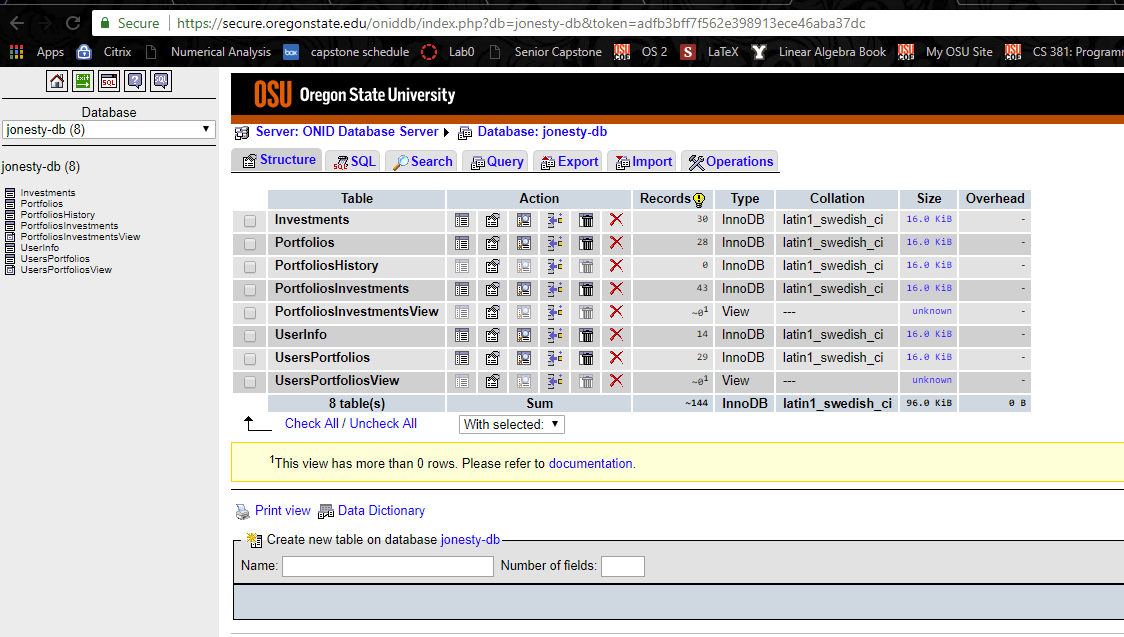
\includegraphics[width=\textwidth]{database_overview}
\end{figure}
A many to many relationship, as I have learned as I have been building my database, is best fixed by adding a 3rd joining table for the relationship. As is demonstrated by the screenshot of all the tables in my database, the naming conventions I have set up, for instance with UsersPortfolios, allows the relationship between multiple users and multiple portfolios to be achieved within the context of a relational database like MySQL. The same goes for PortfoliosInvestments when showing the multiple investments that make up a portfolio. Without going into too much detail, how the process will work, and is working currently, will be that when a user adds a new portfolio, our application will make a call to the API and push the information about that portfolio, including portfolio name and total amount invested in the portfolio into the Porfolios table, as well as insert a new entry into the UsersPortfolios table that specifies who owns that new portfolio, which could be one or multiple users. All of the data that will be queried from the database is from the pictured UsersPortfoliosView, which places all of the portfolios and their owners into a single table, or technically a view in this case, that is able to be queried by our API effectively. This same strategy is applied in the PortfoliosInvestments table, and will also have a corresponding view that allows for effective queries. 

I was overall in charge of two more major components. The first of these components was the API that would communicate with our database. This was a simple php based web api that is housed on my engr web space that permits the user to either return the contents of a table in json format, or upload values to the database when needed within the mobile application. As stated in my previous progress report, I had never worked with API's coming into this term, so having to teach myself the concept was a significant amount of ramp up time. This REST web API is based in php and returns JSON for our C\# based application to parse and display for the user.  The API is generalized so that calls are made to it in the form of “…/api.php/{TableName}”, the output from such a URL is JSON of all the content of the desired table. I felt that making my API simple enough so that calls to it can be generalized and simply return all the content from the table allows me to do my complexities involving the data  through the database and client side, rather than getting bogged down in making an overly complex API. However, reflecting on what I know now, I would navigate away from this API. It ended up being sufficient for our needs for the project, but I have learned a lot since we first used it for our implementation, and I know of many different or better things I would want to attempt with it going forward.

The second major component of this project that was mine to handle was the console application that dynamically calculates user portfolio ratios. This application is a C\# based .Net framework application that communicates with the Alpha Vantage API. This API provides us with our stock pricing data. The portfolio level ratios that we care about are Sharpe Ratio, Alpha, and returns. The main intent of this application was to provide us with a way of conveniently circumventing the significant overhead that goes into each of these calculations. The console application makes an API call for the given portfolios that are in the database, and then runs a considerable amount of calculations on both the portfolios and the pricing data for the companies that are in the portfolio to ultimately reupload the listed ratios to the database again. 

\subsection{What's left to do}

Currently, there is nothing really left to do regarding the user data portions of our application. The database has been configured to our standards, and is properly serving the purpose we need for our user data that is displayed within our mobile app.

\subsection{Problems impeding progress/Solutions}

The biggest problem that we have had thus far, other than personal bottlenecks with having to ramp up our own knowledge of the technical portions, is client issues. At the start of this term, Ron and Edison, our clients, bailed out on the project. Ron left the company, and Edison said it was perhaps best to stop our calls for the time being. This wasn't so much a wrench in the project, as close to all of the work had been done by the time this happened, but was rather just a morale blow that has made the project feel aimless since it now doesn't really have a client that it's being produced for.

\section{Conclusion}
The project has taken a long time to produce, with many hours of work going into every portion of the project. Looking back, this has been an incredible learning experience. Every single component of the application was an entirely new piece of technology for all of us that required a great amount of time and self teaching to use properly. Whether it was C\#, mobile applications, databases, PHP, third party web APIs, or asynchronous code, everything presented its own challenge that needed to be overcome. Moreover, this project has suffered greatly from client consistency. From Brice, our original client, dropping out in Fall term, to the change that just occured with Ron and Edison, it has required a great amount of self discipline and focus to complete this project considering the numerous challenges that we encountered. Overall, however, it has been a very rewarding experience and we are proud of the final product!


\end{document}
